\section{Kryptographie}
%
%
%
\subsection{Ziel:}
Anna und Bruno wollen vertrauliche Nachrichten austauschen. Jedoch ist der Übertragungsweg unsicher. Sie wissen, dass der böse Lasko lauschen wird. Gibt es eine sichere Verschlüsselungsmethode?
%
%
%
\subsection{Problem:}
Alle klassischen Verfahren (z.B. Caesar-Verschlüsselung) arbeiten mit einem geheimen Schlüsselwort, welches von Anna und Bruno zuvor vereinbart werden muss. Insbesondere bei häufigem Wechsel des Schlüsselworts ist das schwierig, da persönliche Treffen in aller Regel zu aufwendig sind. 
%
%
%
\subsection{Erinnerung:}
Sei $0 < a \in \mathbb{R}$ fest. Die \underline{Logarithmusfunktion} $\log_{a}: ]0, \infty [ \rightarrow \mathbb{R}$ zu Basis $a$. ist die Inverse der Abbildung $a^{\BNccc}: \mathbb{R} \rightarrow ]0, \infty [$ speziell $a = e$ \ $x \rightarrow a^{x}$ für alle $ x \in \mathbb{R}$ liefert $ a^{\BNccc} = exp (\BNccc)$ \ $a^{x} = y \leftrightarrow x = \log_{a} y$ \\

\begin{figure} [H]
	\centering
	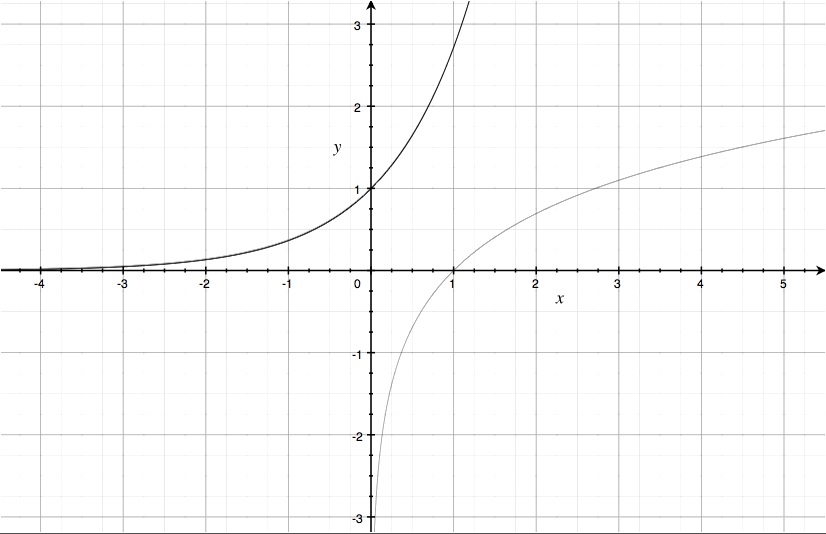
\includegraphics[width=12cm, height=8cm]{mainmatter/chapter2/pics/graphkryp.png}
	\caption{Es wurden $y_{1}= e^{x}$ und \pgrey{$y_{2}=\ln x$}} 
\end{figure}
%
%
%
\subsection{Definition:}
Es seien $ 2 \leq n \in \mathbb{N}$ und $0< a < n$ \underline{fest} gewählt. Gilt $a^{k} \equiv_{n} b$, so nennen wir $k$ einen \underline{diskreten Logarithmus} von $b$ zur Basis $a$ modulo $n$. 
%
%
%
\subsection{Beispiel:}
$n = 13$ \ $a = 7$\\
\qquad\\
\begin{tabular}{c|cccccccccccc} 
$b$ & 1 & 2 & 3 & 4 & 5 & 6 & 7 & 8 & 9 & 10 & 11 & 12 \\\hline 
$\log_{a} b$ mod $n$ & 12 & 11 & 8 & 10 & 3 & 7 & 1 & 9 & 4 & 2 & 5 & 6\\
\end{tabular} 
%
%
%
\subsection{Idee:}
\begin{description}
	\item[-] Die Abbildung $k \rightarrow a^{k}$ mod $n$ ist relativ rasch zu berechnen (vgl. 3.7).
	\item[-] Die Umkehrfunktion, des diskreten Logarithmus erlaubt mit heutigen Methoden keine systematische rasche Berechnung. 
\end{description}
Wir nennen daher $k \rightarrow a^{k} $ mod $ n$ eine Einwegsfunktion.
%
%
%
\subsection{Rasche Berechnung von  $\mathbf{a^{k}}$ mod $\mathbf{n}$}
Sei $k = \varepsilon_{0} \cdot 2^{0} + \varepsilon_{1} \cdot 2^{1} + \dotsc + \varepsilon_{s} \cdot 2^{s}$ mit $\varepsilon_{i} \in \{0,1\} = \sum \limits^{s}_{j = 0} \varepsilon_{j}2^{j}$ die eindeutige Binärdarstellung von  $k$.\\
Dann gilt:
\begin{equation*}
a^{k} = a^{\sum \limits^{s}_{j = 0} \varepsilon_{j}2^{j}} = \prod \limits^{s}_{j = 0} a^{\varepsilon_j s^{j}} = \prod \limits^{s}_{j=0}(a^{2^{j}})^{\varepsilon_j} = \prod \limits^{s}_{\varepsilon_{j = 1}} a^{2^{j}}
\end{equation*}
Wir berechnendaher die $a^{2^{j}}$ mod $n$ durch sukzessives Quadrieren und sofortiges Reduzieren modulo $n$.\\
\qquad\\
\underline{Beispiel:}\\
Berechne $3^{48}$ mod $23$: Dazu: $48 = 32 +16 = 2^{5} + 2^{4} = (110000)_{2}$
\begin{equation*}
	\begin{tabular}{c|c|c|c|c|c|c} 
		$j$ & $0$ & $1$ & $2$ & $3$ & $4$ & $5$ \\\hline 
		$3^{2^{j}}$ \ mod$_{23}$ & $3$ & $9$ & $81\equiv 12$ & $144 \equiv 6$ & $36  \equiv 13$ & $169 \equiv 9$\\
	\end{tabular} 
\end{equation*}
\underline{Fazit:}\\
Anstelle von $48$ Multiplikationen genügen $6$ Multiplikationen. \\
Schlüsseltauschalgorithmus ( Diffie-Hellmann)
\begin{description}
	\item[-] Anna \& Bruno vereinbaren öffentlich eine Primzahl $p$ und eine Basis $a \in \{2,\dotsc, p-2\}$
	\item[-] Anna \& Bruno wählen jeder für sich eine persönliche Geheimzahl $k_{A}$ bzw. $k_{B}$. 
	\item[-] Beide berechnen insgeheim $a^{k_{A}}$ mod $p = b_{A}$ bzw. $a^{k_{B}}$ mod $p=b_{B}$
	\item[-] Anna sendet $b_{A}$ an Bruno, Bruno sendet $b_{B}$ an Anna (öffentlich)
	\item[-] Nun können beide für sich den Rest $a^{k_{A}k_{B}}$ mod $p$ berechnen. 
\end{description}
Da\\
$a^{k_{A}k_{B}} = (a^{k_{B}})^{k_{B}} \equiv_{p} b_{A}^{k_{B}} \leftarrow$ Bruno!\\
$(a^{k_{B}})^{k_{A}} \equiv_{p} b_{B}^{k_{A}} \leftarrow$ Anna!\\
Damit haben beide die Geheimzahl $a^{k_{A}k_{B}}$ mod$p$ vereinbart
\begin{description}
	\item[-] Carlo kennt das ganze System, er kennt $a,p,b_{A},b_{B}$ und kann trotzdem nicht $a^{k_{A}k_{B}}$ mod$p$ berechnen.
\end{description}
%
%
%
\subsection{Definition:}
Es sei T eine Menge an Teilnehmern in einem Netzwerk.\\
Ein \underline{System öffentlicher Schlüssel} sei eine Familie $\{f_{t},g_{t}|t\in T\}$ von Abbildungen derart, dass gilt:
\begin{description}
	\item[-] $f_{t}$ ist eine öffentlich bekannte Einwegsfunktion
	\item[-] $g_{t}$ ist eine nur dem Teilnehmer $t$ bekannte Inverse zu $f_{t}$
\end{description}
%
%
%
\subsection{Definition:}
$T =$ Menge der Teilnehmer $ \{f_{t}, g_{t}|t \in T\}$ wo $f_{t}$ Einwegsfunktion mit Inverser $g_{t}$\\
 \underline{ System öffentlicher Schlüssel}
%
%
%
\subsection{Vorteile:}
\begin{description}
	\item[-] Gibt es ein solches System, in dem jeder Teilnehmer seinen Schlüssel $f_{t}, g_{t}$ selbst bestimmen kann, so entfällt der Schlüsseltausch.
	\item[-] Neue Teilnehmer können jederzeit hinzustoßen.
	\item[-] Spontane Kommunikation wird möglich
	\item[-] $n$ Teilnehmer benötigen lediglich $2\cdot n$Schlüssel. (anstelle $\frac{n(n-1)}{2}$ Schlüssel für Paare von Teilnehmern
\end{description}
%
%
%
\subsection{RSA-Verfahren}
\begin{enumerate}
	\item Schlüsselerzeugung
	\begin{description}
		\item[-] Teilnemer $t$ wählt zwei froße PRimzahlen $p_{t} \neq q_{t}$ und bildet $n_{t} = p_{t} \cdot q_{t}$. 					Dann berechnet $t$ die Eulersche $\varphi$ - Funktion $\varphi (n_{t})$\\
				Dies ist ganz einfach:\\
				Die einzigen Teiler $d \in \{1, \dotsc, n_{t-1}\}$ mit $ggT(d,n) \neq 1$ von $n_{t}$ zwischen $1$ 					und $n_{t}-1$ sind von der Form $p_{t} \cdot a$ (a geeignet ( $1 \leq a \leq q_{t} - 1$ )) oder 					$q_{t} \cdot b$ (b geeignet ( $1 \leq b \leq p_{t} - 1$))\\
				$\Rightarrow$ Es gibt genau ($q_{t} - 1$) + ($p_{t} - 1$) solche $d$.\\
				$\Rightarrow \varphi(n_{t}) = |\{ c | 0 <  c < n_{t},$ $ggT(c_{t},n_{t}) = 1\}| = (n_{t} - 1) - 					(q_{t} - 1) - (p_{t} - 1) = (p_{t} - 1)(q_{t} - 1)$
		\item[-] Nun wählt $t$ eine Zahl $k_{t} \in \{2, \dotsc, \varphi(n_{t}) -1\}$ teilerfram zu $\varphi(n_{t})$ (z.B. 					eine Primzahl $> \varphi(n_{t})$ reduziert modulo$\varphi(n_{t})$)
		\item[-] Mit dem erwarteten Euklid- Algorithmus bestimmt $t$ Zahlen $l_{t}$ und $v_{t}$ so dass $1 = k_{t} 					\cdot l_{t} + \varphi(n_{t}) \cdot v_{t}$
		\item[-] $t$ vernichtet vorraussichtlich $p_{t}, q_{t}, \varphi(n_{t}), v_{t}$ 
		\item[-] als öffentlichen Schlüssel gibt $t$ das Paar $(k_{t},n_{t})$ heraus $i$ als Geheimschlüssel verbleibt $l_{t}$ bei $t$. 
	\end{description}
	\item Die Sicherheit des Verfahrens beruht darauf, dass es für große $p_{t}, q_{t}$ keinen raschen, systematischen 			Weg gibt, um aus $n_{t}$ heraus $p_{t}, q_{t}$ oder $\varphi(n_{t})$ zu bestimmen.
	\item Kryptographie mittels RSA\\
		Anna will Bruno eine nachricht senden. Der Klartext sei eine große ganze Zahl. $x \in \{2, \dotsc, n_{B}-2\}$ (alle 
		ASCII-Zeichen einer Nachricht können in einer einzigen großen Zahl zusammengefasst werden.
	\begin{description}
		\item[-] Anna verschatt sicht den öffentlichen Schlüssel ($k_{b},n_{b}$) von Bruno
		\item[-] Bruno berechnet $z \equiv y^{l_{B}}$ mod$n_{B}$
		\item[-] Nach Satz von Euler (2.9) gilt: \\
				$z \equiv y^{l_{B}} \equiv x^{k_{B}l_{B} + v_{t} \varphi(n_{B})} \equiv x^{1} \equiv$ 						mod$n_{B}$
		\item[-] Es ist extrem unwahrscheinlich dass $ggT(x,n_{B}) \neq 1$ ist, da Anna sonst eine Zerlegung von 						$n_{B}$ gefunden hätte.
		\item[-] Carlo ist machtlos, da er aus $y, k_{B}, n_{B}$ nicht auf $x$ kommen kann, obwohl er das Verfahren 					genau versteht.
	\end{description}
\end{enumerate}
%
%
%
\subsection{elektronische Unterschrift}
Bruno will Anna einen unterschriebenen = authentifizierten Geheimauftrag x senden. Er sendet $y \equiv x^{k_{A}}$ mod$n_{A}$ und zugleich $z \equiv y^{l_{B}}$ mod$n_{B}$\\
Jeder kann verifizieren, dass die verschlüsselte Nachricht von Bruno stammt, indem er $y$ mti $z^{k_{B}}$ mod$n_{B}$ vergleicht. Denn nur Bruno war in der Lage, $z$ aus $y$ heraus zu berechnen.